\pdfoutput=1
\documentclass{llncs}
\usepackage[T1]{fontenc}
\usepackage{newtxtext}
\usepackage[varvw]{newtxmath}
\usepackage{graphicx}
\usepackage{booktabs}
\usepackage{placeins}
\usepackage{amsmath}
\usepackage[hidelinks]{hyperref}
\pdfmapfile{+newtx.map}
\pdfmapfile{+qtm.map}
\pdfmapfile{+txfonts.map}
\pdfmapfile{+cm.map}
\hypersetup{pdftitle={Auditable Solar-Access Decision Support through Exact Blocker Reuse and Containment-Constrained Translation},pdfauthor={},pdfsubject={Anonymous regular-paper manuscript for author review},pdfkeywords={solar access, decision support, exhaustive screening, geometry validation},pdfcreator={LaTeX}}
\pdfinfoomitdate=1
\pdftrailerid{}
\newcommand{\aidraft}{\footnote{Drafting and editing assisted by an OpenAI assistant~\cite{openai2026}; see the AI-Assistance Disclosure.}}
\newcommand{\ind}{\mathbf{1}}
\begin{document}
\title{Auditable Solar-Access Decision Support through Exact Blocker Reuse and Containment-Constrained Translation}
\author{}
\institute{}
\maketitle
\begin{abstract}
Early-stage solar-access decisions require efficient comparison of interventions and reliable translation of simplified rules into geometry. We study a bounded decision-support workflow that selects two of 36 eligible building groups in a 45-building canonical model, giving 630 uniform-height-reduction candidates. Building-level occlusion reuse evaluates every candidate with the same ray--footprint primitive as repeated intersection, while a separate containment audit checks translated stepback solids. Across three matched single-thread repeats, full-universe median runtimes are 11,608.183~s for repeated intersection and 24.037~s for reuse, including precomputation, with equivalent pointwise exposure, metrics, scores, ranks and Pareto results. This 482.927-fold ratio applies to these two implementations, not to arbitrary solar-analysis software. Frozen same-site comparison cohorts of 23 and 20 candidates show strong aggregate agreement with archived Honeybee/Radiance results; the 20-candidate low-sun-area mean absolute error is 0.45~m$^2$, arising from one 9~m$^2$ grid-cell discrepancy. Six controlled historical replays identify outside-footprint walls as the cause of adverse sunlight changes. Four separately simulated contained corrections remove those adverse events on the fixed grid and rays. The canonical geometry remains a component-bounding-box approximation with overlapping footprints. The contribution is an auditable computational screening and translation workflow, conditional on that model, rather than as-built validation or an automatically approved design. Drafting and editing assistance is disclosed for this abstract and the paper~\cite{openai2026}.
\keywords{Decision support \and Solar access \and Exhaustive screening \and Occlusion reuse \and Geometry containment}
\end{abstract}

\section{Introduction}
Solar access is both an environmental performance concern and a constraint on changes to urban form.\aidraft{} A decision-support system must make the comparison of alternatives computationally manageable without obscuring what its model actually represents. Urban solar analysis encompasses different quantities, including irradiation, illuminance and duration of direct exposure; these quantities serve different decisions and should not be treated as interchangeable~\cite{compagnon2004urban,czachura2022metrics}. Here the outcome is sampled outdoor direct-sun duration on a fixed receiving grid. It is neither an indoor daylight metric nor a prediction of annual energy production.

Two practical difficulties motivate this work. First, related candidate interventions repeat much of the same occlusion calculation. When only two building heights change, recomputing all geometric intersections for every candidate discards reusable information. Second, an attractive result in a simplified screening model does not guarantee that a subsequently generated design solid implements the intended intervention. A nominally subtractive stepback can inadvertently add material outside the original footprint. Ranking such an invalid translation more carefully does not repair its physical meaning.

We examine these difficulties together in a bounded case study. The decision universe contains all 630 pairs from 36 eligible building groups within a 45-building canonical model. Eligibility is an input constraint for research, not permission to modify a property. Each pair receives a prescribed uniform-height reduction and is evaluated by low-sun grid area, mean direct-sun duration, a nominal volume proxy and newly low-sun grid area. A fixed weighted score expresses preferences; an area--volume Pareto analysis offers a complementary view. Translated stepback geometries are evaluated separately rather than assumed equivalent to the screening rules.

The study addresses three questions. (1) What efficiency gain does building-level blocker reuse deliver against repeated intersection when both implementations use the same primitive, inputs, single-thread execution and output checks? (2) How closely do frozen screening aggregates agree with archived Honeybee/Radiance aggregates within two preserved same-site review cohorts? (3) Can the adverse exposure changes in historical translations be explained by actual ray hits and removed by separately evaluated contained geometry? These questions distinguish implementation efficiency, aggregate agreement and translation validity. None alone establishes real-site accuracy.

The contributions are a bounded formulation with exact blocker reuse, a four-scale comparison including precomputation, and a controlled translation audit retaining negative historical outcomes and evaluating four corrections. Explicit metric, tie and volume semantics connect these results to their limitations. The contribution is an auditable application-specific workflow, not a learned model or a new general optimization algorithm.

\section{Related Work and Positioning}
Urban solar-performance assessment has long considered the interaction between built form and the availability of sunlight and daylight.\aidraft{} Compagnon~\cite{compagnon2004urban} evaluates solar and daylight availability in urban fabric through surface-based performance analysis. The taxonomy of Czachura et al.~\cite{czachura2022metrics} helps distinguish the metrics used in urban planning. This distinction matters here: a threshold on sampled direct-sun hours cannot be substituted for irradiation, daylight autonomy or a jurisdiction-specific compliance test.

Simulation-based design-support methods already connect changes in building form to environmental objectives. Konis et al.~\cite{konis2016passive} present an optimization framework for early-stage passive-design support. De Luca et al.~\cite{deluca2021reverse} develop a reverse solar-envelope form-finding method that can accommodate regulatory frameworks. Our study has a narrower search space: it exhaustively ranks a fixed set of two-building height-reduction rules, then treats stepback generation as a separate, fallible translation. We do not benchmark against those systems or infer that exhaustive enumeration outperforms their broader form-finding methods.

The software ecosystem also supplies distinct computational roles. Ladybug supports parametric environmental analysis~\cite{roudsari2013ladybug}; Radiance provides a lighting simulation and rendering system based on ray tracing~\cite{ward1994radiance}; and pvlib supplies solar-energy modeling implementations including solar-position calculation~\cite{holmgren2018pvlib}. These references establish the context of the tools, not the validity of our particular inputs or recipe. In particular, the effective solar vectors recovered from the archived Honeybee/Ladybug route are not numerically identical to the saved pvlib vectors. Cross-route agreement therefore concerns the actual archived configurations, whereas the efficiency comparison isolates two implementations using exactly the same geometric primitive and vectors.

\section{Decision Model and Exposure Estimator}
\subsection{Bounded Candidate Universe}
Let $\mathcal{B}$ denote the 45 building groups, each represented by a footprint $F_i$ and height $h_i$.\aidraft{} The eligible subset $E\subset\mathcal{B}$ contains 36 groups selected using source flags for movable and protected buildings, strict Boolean parsing and $h_i>3$~m. A feasible rule decision satisfies
\begin{equation}
 z_i\in\{0,1\}\ (i\in E),\qquad \sum_{i\in E}z_i=2,
 \label{eq:select}
\end{equation}
with $z_i=0$ outside $E$. For a selected building, the rule height is
\begin{equation}
 h_i^r=\max\{3,\ h_i-\min(3,0.25h_i)\},\qquad
 h_i(z)=(1-z_i)h_i+z_i h_i^r, \label{eq:height}
\end{equation}
where heights are in metres. Thus $\binom{36}{2}=630$ unordered pairs constitute the complete declared universe. Exhaustive evaluation establishes an optimum only for a specified score within this finite universe. It says nothing about other numbers of altered buildings, alternative height rules, footprint changes, structural feasibility or legal rights.

The canonical footprints are unions of bounding boxes associated with DXF components. Some building identifiers share components and some footprints overlap. The archived OBJ representation also disagrees with the canonical model for important candidates. We retain the frozen canonical input for reproducibility, but do not describe it as a surveyed or as-built boundary model. This distinction affects both visibility and volume interpretation.

\subsection{Receiving Grid, Time Samples and Visibility}
The protocol fixes 2,031 receiving points on a 3~m horizontal grid at height 0.1~m. The geographic parameters are latitude $24.55^\circ$N and longitude $118.03^\circ$E, with UTC+8 local time and an assumed north angle of zero. The declared analysis date for the pvlib sequence is 21 December 2026. Sixteen half-hour samples are centred at 08:15, 08:45, $\ldots$, 15:45. Each carries weight $\Delta t=0.5$~h, so the total integration weight is 8~h, despite the 7.5~h span between the first and last sample centres. These are discrete samples, not continuous-time exposure measurements.

For receiver $j$ and sample $t$, let $d_t=\ind\{\alpha_t>0\}$ indicate an above-horizon solar altitude and let $b_{jt}(z)$ indicate obstruction by at least one building. Direct-sun duration is
\begin{equation}
 D_j(z)=\sum_{t=1}^{T}\Delta t_t\,d_t\,[1-b_{jt}(z)].
 \label{eq:dsh}
\end{equation}
The geometric primitive intersects a horizontal ray with a footprint and uses the first positive projected distance $\ell$ to compare the ray height $0.1+\ell\tan\alpha_t$ against the building height. The source primitive ignores distances at most $10^{-7}$~m and uses a $10^{-9}$~m height tolerance. Point ordering, footprint construction, direction convention, tolerances and solar vectors are held identical in the matched comparison. The actual canonical case has no polygon holes; all receiving points were verified outside the canonical building footprints and off their boundaries. Those case-specific checks do not establish correctness for arbitrary polygon holes or boundary configurations.

The explicit active-sun factor in Eq.~\ref{eq:dsh} is important. A reproduced latent defect in the legacy routine skips constructing below-horizon rays but then counts their unblocked entries as visible. All 16 saved samples are above the horizon, so this defect is not evidence of a wrong frozen exposure value. It is nevertheless a reason to require an active-sun mask for extensions to other schedules.

\subsection{Metrics and Preferences}
Let $D_j^0$ be baseline duration, $P=2031$, $a=9$~m$^2$ the grid-area weight and $\tau=3$~h the research threshold. Four candidate metrics are
\begin{align}
 A(z)&=a\sum_j\big[\ind\{D_j^0<\tau\}-\ind\{D_j(z)<\tau\}\big],\label{eq:area}\\
 H(z)&=P^{-1}\sum_j[D_j(z)-D_j^0],\label{eq:hours}\\
 V(z)&=\sum_i |F_i|[h_i-h_i(z)],\label{eq:volume}\\
 N(z)&=a\sum_j\ind\{D_j^0\geq\tau,\ D_j(z)<\tau\}.\label{eq:new}
\end{align}
Here $A$ is net reduction of low-sun grid area, $H$ is mean duration change, $V$ is the nominal per-building volume proxy and $N$ is newly low-sun grid area. In a model with nonoverlapping fixed-footprint prisms, Eq.~\ref{eq:volume} measures removed volume. With the present overlapping footprints it is an additive proxy, not actual whole-scene net union-volume reduction or a construction quantity. Translated solids require a separate net union-volume calculation. The 3~h threshold defines this analysis; no statutory status is claimed.

For each $q\in\{A,H,V,N\}$, normalization bounds are fixed from the full 630-rule universe:
\begin{equation}
 n_q=\begin{cases}(q-q_{\min})/(q_{\max}-q_{\min}),&q_{\max}-q_{\min}\geq10^{-12},\\0,&\text{otherwise}.\end{cases}
 \label{eq:norm}
\end{equation}
The preference score is
\begin{equation}
 S=0.45n_A+0.35n_H+0.15(1-n_V)+0.05(1-n_N).
 \label{eq:score}
\end{equation}
The weights are declared preferences, not learned parameters or probabilities. Bounds are not refitted to the review cohorts or Honeybee outcomes, and out-of-range values are not silently clipped. Table~\ref{tab:bounds} reports the frozen bounds. All rule candidates have $N=0$; hence the final term contributes a constant 0.05 and has no discriminating power in this universe. Changing only its weight cannot change the ordering. A historical sensitivity scenario that also changed the $A/H$ weights does not isolate the effect of $N$.

\begin{table}[tbp]
\caption{Full-universe normalization bounds. $V$ is a nominal additive proxy.}
\label{tab:bounds}\centering
\begin{tabular}{lrrl}\toprule
Metric & Minimum & Maximum & Unit\\\midrule
$A$ & 0 & 396 & m$^2$\\
$H$ & 0 & 0.06351551 & h\\
$V$ & 387.38244 & 10,891.47442 & m$^3$\\
$N$ & 0 & 0 & m$^2$\\\bottomrule
\end{tabular}
\end{table}

Candidates are sorted deterministically by score and the specified pair-order tie rule. The accompanying Pareto analysis maximizes $A$ and minimizes $V$, with at least one strict improvement required for domination. It is a two-objective front, not a four-objective optimization. A high score, Pareto membership, geometric validity and professional acceptability remain different judgments.

\section{Exact Blocker Reuse and Translation Checks}
\subsection{Reusable Building Contributions}
For each building $i$, receiver $j$ and time $t$, precompute Boolean occlusion arrays $O_{ijt}$ and $R_{ijt}$ at the original and rule-reduced heights using the common primitive.\aidraft{} Let $C_{jt}=\sum_i O_{ijt}$ be the original number of blockers. For selected pair $(a,b)$,
\begin{align}
 C_{jt}^{(a,b)}&=C_{jt}-O_{ajt}-O_{bjt}+R_{ajt}+R_{bjt},\label{eq:reuse}\\
 b_{jt}^{(a,b)}&=\ind\{C_{jt}^{(a,b)}>0\}.\label{eq:block}
\end{align}
These updates use a signed integer count type sufficiently wide for the building count. Subtraction in Boolean or unsigned storage can silently corrupt counts and is not an acceptable implementation of Eq.~\ref{eq:reuse}.

The identity follows directly by partitioning the sum of building blockers into the two selected buildings and the unchanged remainder. Removing the original contributions of $a,b$ and adding their reduced-height contributions yields the same count as recomputing every building contribution. The threshold in Eq.~\ref{eq:block} then gives the same visibility. This is an algebraic equivalence conditional on identical primitive outputs, independent building contributions and unchanged unselected geometry. It does not equate the primitive to a different ray tracer, nor does it apply to a translated footprint merely because that translation shares a candidate label.

The implementation validates ordered inputs, computes the two blocker arrays and baseline counts, streams the pair updates into Eq.~\ref{eq:dsh}, and derives Eqs.~\ref{eq:area}--\ref{eq:new}. Scores use fixed full-universe bounds, followed by deterministic ranking and the $A/V$ Pareto scan. Streaming avoids storing a full candidate--receiver--time cube. Geometry, time and candidate identities accompany the aggregate outputs so that a later score is not detached from the model that produced it.

\subsection{Computational Cost and Accounting}
Let $B,P,T,M$ be the building, receiver, time-sample and candidate counts, and let $G$ denote the cost of a ray--footprint intersection. Repeated candidate intersection has work of order $O(MBPTG)$ before early exits. Reuse requires $O(BPTG)$ preparation and $O(MPT)$ candidate updates and metrics. Polygon complexity and possible indexing affect $G$; it is not a universal constant. Score sorting adds $O(M\log M)$ and the present direct Pareto scan adds $O(M^2)$ comparisons.

Two byte-valued blocker arrays require $2BPT$ bytes. At the present dimensions this is 2,924,640 bytes, approximately 2.79~MiB. This analytic storage count excludes geometry, solar data, integer count arrays, temporaries, indexes and Python overhead. It is not measured peak process memory. Input preparation, precomputation, candidate processing and output costs must be included consistently when evaluating actual efficiency.

We therefore compare two specific implementations: A repeats the primitive for each candidate, retaining first-blocker short-circuiting; B precomputes building blockers and reuses them. Neither implementation uses a spatial index in this experiment. B's end-to-end runtime includes independent precomputation for each repeat. A warm-cache update-only time would answer a different question and is not used as the denominator of the reported speedup.

\subsection{Containment as a Physical Invariant}
Let $\Omega_0$ be the baseline opaque solid and $\Omega_c$ a translated candidate solid. A genuine subtraction satisfies $\Omega_c\subseteq\Omega_0$. For fixed receiving points and solar rays, a ray unobstructed by $\Omega_0$ cannot become obstructed by a subset of $\Omega_0$. Thus containment implies nondecreasing sampled direct-sun exposure. An adverse event under these assumptions requires examination of geometry, ray mapping, receiving-point mapping or computation; it cannot simply be justified as an unavoidable trade-off of subtraction.

Historical stepback generation is therefore audited independently of score ranking. The audit checks containment of generated solids, preservation of expected faces, actual ray intersections for adverse visibility events, and whole-scene union volumes. The corrected generator constrains the translated geometry to the original solid footprint and is evaluated in separate runs. Containment is not volume matching: clipping an outside region may change the amount removed, and overlapping building footprints make per-building sums differ from scene-union differences. We preserve both the original and corrected outputs rather than replacing the history with the favorable result.

\section{Experimental Protocol}
\subsection{Evidence Layers and Frozen Inputs}
Three evidence layers are kept separate.\aidraft{} The matched implementation experiment uses the canonical real-case input and the complete fixed candidate order. The same-metric agreement study recomputes statistics from frozen archived aggregates for a curated cohort of 23 and a separately preserved coverage cohort of 20. Finally, controlled Honeybee/Radiance replays revisit a baseline and five historical translations, followed by four corrected scenes. The original 20-candidate sample is neither reselected nor rerun in the correction experiment.

The coverage cohort was selected for score-stratum, volume and identifier coverage and held out from curated review. It is an outcome-blind same-site coverage sample, not a probability sample or an independent site. Archived timestamps report freezing before its Honeybee execution; a file hash verifies unchanged bytes but does not by itself prove that chronology. We use descriptive agreement measures without a population-generalization claim.

A pre-benchmark amendment repaired a normalization-source hash mismatch, pinning the actual committed bytes and an independent frozen reference. All 630 candidate identities and metrics agreed within existing tolerance. The original failed check was retained; score bounds were not adapted to outcomes.

\subsection{Matched Runtime and Equivalence}
The runtime experiment uses nested fixed prefixes of 5, 20, 60 and 630 candidates, with three measured A/B repeats at each size. Warm-up and pilot runs are excluded from the reported medians. Each comparison fixes geometry, ordered receivers, solar vectors, tolerance, candidate order, score bounds and phase accounting. Equivalence is checked for pointwise duration, $A/H/V/N$, scores, ranks and Pareto membership before reporting runtime ratios. The 630-candidate A runs were completed; their times are measured rather than extrapolated.

The environment is Windows 11, Python 3.12.2, NumPy 2.4.6, Shapely 2.1.2 with GEOS 3.13.1, and pvlib 0.15.2. The processor is recorded as AMD64 Family 25 Model 80 Stepping 0, with 16 logical CPUs available. The experiment uses one process and one thread; common numerical-library thread environment variables are fixed to one. Elapsed time is measured with \texttt{time.perf\_counter}. The record does not supply a verified commercial CPU model name, and unavailable Windows resident-set measurements are left unknown rather than reported as zero.

\subsection{Cross-Route Agreement and Temporal Audit}
Within each preserved cohort, the screening route is compared to the archived Honeybee route using the same metric on both sides: $A$ with $A$, $H$ with $H$ and $S$ with $S$. Scores use unchanged full-universe bounds. We report Spearman correlation with average ranks for ties and candidate-level mean absolute error (MAE). Shared $V$ inputs and the constant $N$ term restrict the independence of the composite-score comparison.

Exact-$K$ sets use descending metric followed by natural numeric pair order. The legacy source-row-order tie rule and inclusion of all boundary ties are reported as sensitivities. Every such result belongs to its comparison cohort; no selected-cohort statistic is interpreted as recall across all 630 candidates. Numerical zero p-values are not interpreted as exact probability zero, and significance claims are unnecessary for these nonprobability cohorts.

Actual archived WEA records, hour-of-year labels, solar-source names and all 16 visibility columns were reconciled across the six historical scenes. Every cumulative exposure equals its binary visibility sum multiplied by 0.5~h. The WEA inputs have constant direct-normal irradiance of 1000~W/m$^2$ and diffuse-horizontal irradiance of zero. They carry the direct-sun-hours analysis rather than measured weather. WEA/hour-of-year records lack a calendar-year field, so the archived Ladybug reconstruction is not an identical year-specific astronomical input to the declared 2026 pvlib sequence. Effective rays are shared across the controlled historical scenes but differ measurably from the saved pvlib rays. North zero remains an assumption.

\subsection{Controlled Translation Replays}
Six controlled replays comprise the baseline and five historical translated pairs: C9/C24, C9/C15, C9/C13, C13/C24 and C6/C33. Their ordered receiver grid, solar sources, time columns and archived scene identity are checked. New runs use one CPU and one worker. All six reproduce their historical pointwise visibility matrices exactly. Four contained corrections are then simulated separately. C9/C13 was already contained and is not simulated again as a correction; its unchanged value is reused only for comparison. There are therefore ten new scene runs, not eleven, and no full 630-scene Honeybee experiment.

\section{Results}
\subsection{Measured Reuse Efficiency}
All 12 measured scale/repeat comparisons pass pointwise and aggregate equivalence checks.\aidraft{} Table~\ref{tab:runtime} and Fig.~\ref{fig:runtime} report the scale-level medians. At 630 candidates, repeated intersection takes 11,608.183~s and reuse takes 24.037~s including precomputation; their ratio is 482.927. The relative benefit increases with the candidate count as repeated geometry work accumulates while preparation is amortized.

\begin{table}[tbp]
\caption{Measured end-to-end runtime medians from three single-thread repeats at each size. B includes precomputation. Ratios compare these implementations only.}
\label{tab:runtime}\centering
\begin{tabular}{rrrrr}\toprule
Candidates & Repeats & A (s) & B (s) & A/B\\\midrule
5 & 3 & 109.706 & 23.359 & 4.697\\
20 & 3 & 373.812 & 23.418 & 15.963\\
60 & 3 & 1,085.983 & 23.975 & 45.297\\
630 & 3 & 11,608.183 & 24.037 & 482.927\\\bottomrule
\end{tabular}
\end{table}

\begin{figure}[tbp]\centering
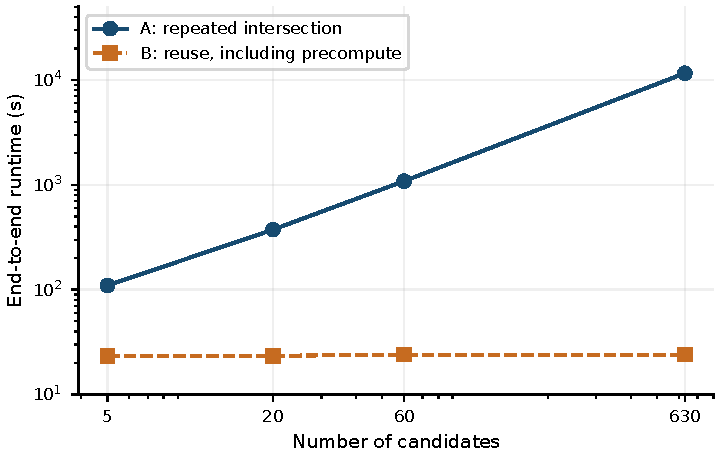
\includegraphics[width=\textwidth]{figures/runtime_publication.pdf}
\Description{Logarithmic plot of measured runtime against candidate count. A rises from approximately 110 seconds at five candidates to 11608 seconds at 630. B remains around 23 to 24 seconds, including precomputation.}
\caption{Measured same-primitive runtime comparison on the frozen canonical model. Both axes are logarithmic; points are medians of three repeats. Pointwise duration, metrics, score, rank and Pareto checks agree. The figure contains aggregate results only.}
\label{fig:runtime}
\end{figure}

This is an implementation comparison, not a general solver comparison. In particular, the repeated-intersection implementation is not a spatial-index baseline, and the experiment does not time equivalent Honeybee scenes against B. Historical screening and Honeybee timings with different machines, solver semantics or worker counts are excluded from the ratio. The result supports the benefit of reuse in the measured setting, while leaving the benefit relative to other optimized implementations unmeasured.

The full-universe regression also preserves the historical candidate order. Differences in $A$, $H$ and $N$ are zero; the maximum absolute $V$ difference is approximately $9.09\times10^{-13}$~m$^3$ and the maximum score difference approximately $4.44\times10^{-16}$, consistent with floating-point rounding. There is no changed 630-candidate ranking. These checks establish consistency with the frozen output, not fidelity of its geometry to the physical site.

\subsection{Agreement within Preserved Cohorts}
Table~\ref{tab:agreement} separates the two cohorts and the three compared metrics. For low-sun-area reduction, the curated cohort has Spearman $\rho=0.999258$ and the coverage cohort $\rho=0.997668$. In the latter, 19 candidates agree exactly and one differs by 9~m$^2$, yielding MAE 0.45~m$^2$. This is an average candidate-aggregate error on a grid with 9~m$^2$ cell weights; it is not sub-grid spatial precision. Figure~\ref{fig:agreement} visualizes the same frozen aggregate comparison.

\begin{table}[tbp]
\caption{Descriptive same-metric agreement with archived Honeybee aggregates. Statistics are recomputed from frozen tables; no new cohort simulations are implied.}
\label{tab:agreement}\centering
\begin{tabular}{llrrr}\toprule
Cohort & Metric & Spearman $\rho$ & MAE & Exact matches\\\midrule
Curated ($n=23$) & $A$ (m$^2$) & 0.999258 & 0.391304 & 22/23\\
 & $H$ (h) & 0.991597 & 0.001177 & 3/23\\
 & $S$ & 0.999012 & 0.006933 & 3/23\\
Coverage ($n=20$) & $A$ (m$^2$) & 0.997668 & 0.450000 & 19/20\\
 & $H$ (h) & 0.999624 & 0.000295 & 9/20\\
 & $S$ & 1.000000 & 0.002139 & 9/20\\\bottomrule
\end{tabular}
\end{table}

\begin{figure}[tbp]\centering
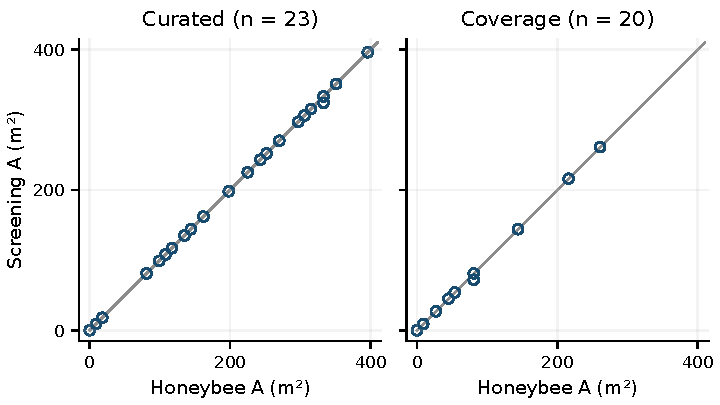
\includegraphics[width=\textwidth]{figures/agreement_publication.pdf}
\Description{Comparison of screening and archived Honeybee low-sun-area reductions, displayed separately for the curated 23 and coverage 20 candidate cohorts. Near-diagonal aggregate agreement does not establish site or pointwise equivalence.}
\caption{Low-sun-area agreement from frozen candidate aggregates. Each cohort remains separate. The coverage cohort's mean absolute difference of 0.45~m$^2$ arises from one 9~m$^2$ discrepancy among 20 candidates.}
\label{fig:agreement}
\end{figure}

Coverage-cohort score ranks agree perfectly, but the score values do not: MAE is 0.002139 and only 9 of 20 scores agree exactly. Moreover, $V$ is shared between routes and $N$ is constant. The score comparison cannot validate four independent performance criteria, and correlation one cannot be read as 100\% predictive accuracy. The exposure routes also have different effective solar vectors. Their high aggregate agreement is useful evidence for this frozen screening task, with those qualifications.

Tie handling materially affects the top-five $A$ comparison within the 20-candidate coverage cohort. Here overlap is divided by five for exact-five sets. The retained legacy source-order result of 0.8 becomes 1.0 under the specified natural-pair exact-five rule, while including all boundary ties produces sets of six and seven candidates. This is a change in set definition, not an improvement in the physical model. We consequently avoid presenting a single top-five overlap as a universal selection guarantee. Likewise, an older correlation that compared score ranks to area ranks is not compared to the present same-metric correlations as evidence of progress.

\subsection{Translation Failure and Controlled Correction}
Four of five historical translations fail the solid-containment check. In C9/C24 and C13/C24, rays that were clear in the baseline intersect upper walls of C24 outside its original footprint. Each of these scenes has four worsened receiving points and 9~m$^2$ of newly low-sun grid area in the retained historical result. The actual ray hits identify added obstructions as the cause. Synthetic tests had also exposed hole-handling and silent-face risks, but the canonical site has no holes and the six archived face dictionaries regenerate exactly; those synthetic defects are not asserted as the cause of this case.

The four contained corrections have no adverse visibility events, worsened receiving points or newly low-sun grid area on the fixed model, rays and grid. Figure~\ref{fig:translation} retains the before/after distinction. Low-sun-area reduction changes from 342 to 351~m$^2$ for C9/C24 and from 207 to 216~m$^2$ for C13/C24. C9/C15 and C6/C33 remain at 342 and 18~m$^2$. The already-contained C9/C13 remains at 333~m$^2$ through reuse of its unchanged historical result, not an additional correction run.

\begin{figure}[tbp]\centering
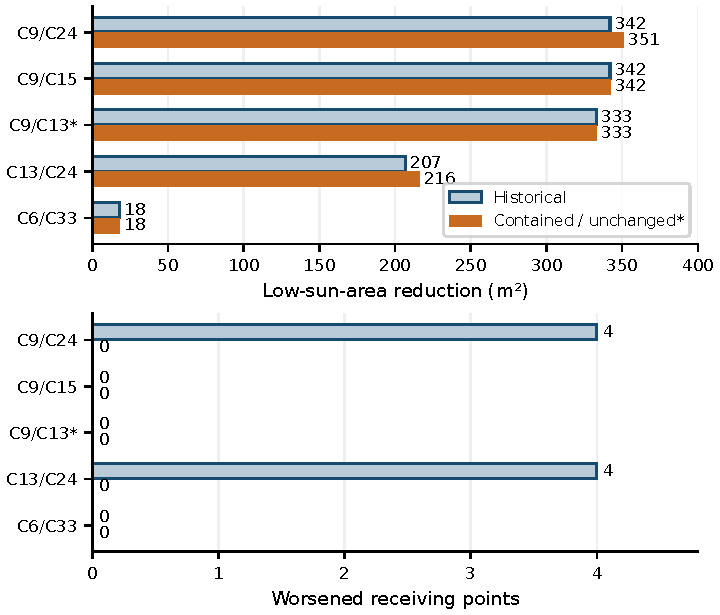
\includegraphics[width=\textwidth]{figures/translation_publication.pdf}
\Description{Five paired historical and corrected displays. C9/C24 and C13/C24 improve area reduction by nine square metres and reduce worsened points from four to zero. The C9/C13 corrected display reuses an unchanged historical result.}
\caption{Controlled translation recheck. Top: low-sun-area reduction relative to baseline. Bottom: worsened receiving-point count. Four corrections are newly simulated; C9/C13 is already contained and reuses its unchanged result. The historical adverse results remain visible; the comparisons are not volume matched.}
\label{fig:translation}
\end{figure}

For any translated solid, the signed net union-volume reduction is $|\Omega_0|-|\Omega_c|$. For a noncontained legacy solid, this equals removed baseline volume minus added outside volume; it is not gross removed material. Table~\ref{tab:volumes} shows why containment correction must not be called a volume-matched comparison. Nominal rule budgets, rule-solid net union-volume reduction and translated-solid net union-volume reduction differ. C6/C33 is particularly informative: its nominal additive proxy is 5,583.055~m$^3$, while uniform-rule net union-volume reduction is 1,909.864~m$^3$ and corrected translation net union-volume reduction is 2,554.767~m$^3$. These quantities characterize the frozen approximate solids, not verified demolition or construction quantities. Similar area outcomes do not imply geometrically equivalent interventions.

\begin{table}[tbp]
\caption{Volume distinctions in the canonical model (m$^3$). The nominal column is additive per building; other columns use signed whole-scene net union-volume reductions. C9/C13's correction column reuses its already-contained result.}
\label{tab:volumes}\centering
\begin{tabular}{lrrrr}\toprule
Pair & Nominal rule & Rule union & Legacy union & Corrected union\\\midrule
C9/C24 & 5,551.333 & 5,470.406 & 5,259.615 & 5,474.582\\
C9/C15 & 3,127.755 & 3,065.681 & 2,927.693 & 2,937.931\\
C9/C13 & 2,975.156 & 2,918.246 & 2,785.422 & 2,785.422\\
C13/C24 & 3,863.880 & 3,726.044 & 3,534.257 & 3,749.224\\
C6/C33 & 5,583.055 & 1,909.864 & 2,553.509 & 2,554.767\\\bottomrule
\end{tabular}
\end{table}

\FloatBarrier
\section{Discussion and Limitations}
\subsection{Implications for Decision Support}
Reuse makes exhaustive comparison inexpensive after building contributions have been prepared.\aidraft{} The bounded universe exposes all candidates, fixed normalization bounds and the area--volume trade-off. Altering the rule, geometry or solar protocol requires new blocker contributions and renewed checks.

The translation result is equally important for decision support. A scoring system can be internally consistent while a downstream geometric representation violates its physical premise. Containment supplies an inexpensive conceptual invariant, and ray-level evidence distinguishes an actual added obstruction from a speculative explanation. Preserving the failed translation alongside the correction prevents an apparent design benefit from erasing the diagnostic evidence. It also makes clear that ranking and translation are separate stages with different acceptance criteria.

The workflow supports shortlisting under a declared model, followed by separate geometric and performance review. Cost, ownership, safety, constructability and regulatory acceptability remain external decisions. The weights are not a validated social preference model; professional use requires verified geometry and stakeholder-specific criteria.

\subsection{Threats to Validity}
\paragraph{Canonical geometry.} The DXF component-bounding-box unions, shared components, overlapping footprints and OBJ disagreements are the most important external-validity limits. Reproducing a canonical model across implementations cannot validate its as-built fidelity. Correcting those boundaries would define a new input version and require an explicit assessment of affected results. Current cohort agreement must not be transferred to that new geometry without evidence.

\paragraph{Restricted physical scope.} A single day, 16 samples, a 3~m grid, a 0.1~m receiving height and an assumed north orientation delimit the reported performance. Threshold counts can change discontinuously near 3~h. The constant WEA carrier is not measured meteorology, and the study does not validate indoor illuminance, glare, annual weather, energy production or regulatory compliance. The distinction between saved pvlib rays and archived Ladybug rays remains part of the cross-route comparison rather than being suppressed to imply identical astronomical inputs.

\paragraph{Comparison design.} The matched timing comparison controls the geometric primitive and single-thread execution, but covers only one canonical model and two implementations without spatial indexing. Three repeats quantify the recorded execution conditions; they do not characterize hardware populations or arbitrary polygon complexity. We do not claim a measured memory reduction from the analytic blocker-array size or unavailable RSS values. A stronger efficiency comparison would include indexed and compiled baselines with the same accounting contract.

\paragraph{Cohorts and metrics.} Curated review and outcome-blind coverage serve different purposes and remain separate. Neither is a random multi-site sample. Shared volume inputs, constant $N$, discretized area, ties and preference weights constrain the interpretation of rank agreement. Candidate-level aggregate errors can mask spatial differences. The frozen 20 were not selectively rerun after the translation audit because no shared receiver, temporal-parser or missing-face defect was found in the actual scenes. A newly demonstrated shared defect would require an affected-scope review rather than selective retention of favorable outputs.

\paragraph{Correction scope.} Four corrected translations remove the observed adverse events under fixed rays and receivers. This supports the tested containment correction on this canonical model, not a guarantee for arbitrary imported meshes. Containment does not ensure equal volume, structural feasibility or a preferred design. The nominal $V$ proxy should be replaced or supplemented by an appropriate audited quantity if the decision requires physical removal costs.

\subsection{Reproducibility and Responsible Release}
The evidence separates measured runtime, newly executed scene replays, frozen-table statistical recomputation and historical reused results. Run identifiers, source, configuration and input hashes, raw timing repeats, aggregate tables, equivalence checks, correction ledgers and figure-source manifests are retained. The final integrated test record contains 112 passing tests; this supports software regression coverage, not physical ground truth. Failures and amendments remain part of the record rather than being overwritten.

Raw CAD, DXF, SKP and OBJ inputs, receiver coordinates, WEA carriers, Honeybee models and Radiance intermediate data remain restricted. Figures in this manuscript show aggregate evidence without site geometry or receiver coordinates. No public artifact release or unrestricted replication right is asserted. Any external evidence package must be reviewed for rights and anonymity before distribution. This restriction limits independent reproduction of the site-specific experiment and should remain visible alongside the available aggregate and algorithmic detail.

\section{Conclusion}
A bounded solar-access screening problem can reuse exact building-level occlusion contributions while keeping its preference model and geometric limitations explicit.\aidraft{} On the frozen 45-building canonical model, all 630 pair candidates are evaluated with equivalent outputs by two same-primitive implementations. Three matched repeats yield median end-to-end times of 11,608.183~s for repeated intersection and 24.037~s for blocker reuse, including preparation. The resulting ratio is specific to those implementations and inputs.

Preserved cohorts show strong same-site aggregate agreement, while controlled replays locate outside-footprint obstructions and remove the observed adverse events in four contained corrections. The results support auditable screening, not as-built accuracy, volume-matched interventions or automatic design approval. Verified boundaries, broader site coverage and additional optimized baselines are the next substantive extensions.

\section*{AI-Assistance Disclosure}
An OpenAI assistant~\cite{openai2026} assisted with evidence organization, drafting and editing the abstract and Sections~1--8, mathematical presentation, table transcription, figure captions and alternative text, bibliography checking, and LaTeX build and quality-control scripts. The manuscript uses reported experimental measurements and frozen aggregates; no numerical observations were generated to fill missing evidence. The assistant also prepared publication-size plots from unchanged aggregate tables. These figures reproduce recorded evidence rather than generative illustrations. This statement describes the assistance used for the present draft. The exact underlying model/version was not recorded, so no model-version claim is made.

\FloatBarrier
\bibliographystyle{splncs04}
\bibliography{references}
\end{document}
